
\section{Implementation}\label{implementation}

In this section, we outline the plan to implement each component of our system as it was designed in the previous section.
Specifically, we are outlining the implementation plan for the trading simulation software required to test the strategies that are being researched and will be implemented in a later stage of this project.
Additionally, the responsibilities for each member of our team will be made clear.

Our team will make use of the Git version control tool to help maintain our project \cite{git}.
We will use GitHub's free web service to host our source code publicly \cite{github}.
This repository is available at \url{github.com/saurabh/cs4624}.

\subsection{Pricing Data}

To recap the design section, the implementation of the pricing data component involves setting up the database schema, implementing an interface that stores and retrieves stock prices (in the data structure described) from our database, and, finally, implementing utilities that request and parse the stock price information from external sources.
The effort behind the implementation of this component is led by Joseph Watts.

\subsubsection{Setting Up Database Schema}

In order to prepare HBase to store our data, we need to define the table that will store the stock prices from a given data source.
With HBase, tables need to be predefined with a name and a list of column families before they can be used to store any information \cite{hbase}.
In this case, the name of our table will correspond to the stock prices that we are storing (for example, \texttt{dailystockprices}).
Then, this table will contain one column family named \texttt{price}.
To actually execute the command that defines this table in the database, we first start the HBase shell by running \texttt{hbase shell}.
Then we run the command \texttt{create 'dailystockprices','prices'} in this shell.

\subsubsection{Database Interactions}

Assuming that a table to hold stock prices is predefined, we need interfaces to query stock prices from this table and write stock prices to this table.
\texttt{StockPriceDataSource} (see figure~\ref{stockPriceDataSource}) is a Scala trait (which is similar to an interface in Java) that abstracts away the actual source of the stock prices.
All objects that implement \texttt{StockPriceDataSource} must define two methods that allow you to request stock prices.
The \texttt{query} method allows you to do a range query for stock prices of a particular symbol between two timestamps.
The \texttt{priceAtTime} method allows you to get the most recent stock price of a particular symbol (that is, on or before a given timestamp).
\texttt{StockPriceDataSource} affords this system the flexibility of moving away from HBase towards a different database solution.
We define a \texttt{HBaseStockPriceDataSource} class which implements the contract laid out by \texttt{StockPriceDataSource}.
The constructor for the \texttt{HBaseStockPriceDataSource} class takes the table name as a parameter.
\texttt{HBaseStockPriceDataSource} provides functions that write stock prices back to the source (the database).
These functions are used by the tools which query the external sources and populate HBase with their data.

% Figure - stockPriceDataSource
\begin{figure}[h]
  \label{stockPriceDataSource}
  \begin{center}
    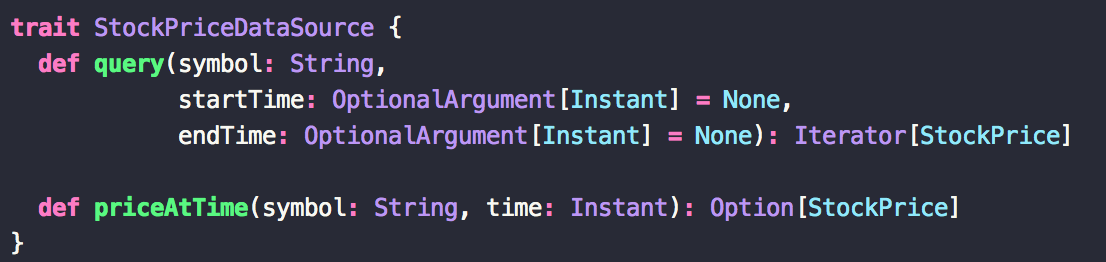
\includegraphics[max width=\textwidth]{stockPriceDataSource}
  \end{center}
  \caption{The \texttt{StockPriceDataSource} trait.}
\end{figure}

\subsubsection{External Sources}

We use two different external sources to retrieve daily stock prices for the full set of stocks of interest.
This set of securities consists of the 11 stocks in Table~\ref{tab:stocks} and the S\&P 500 index.
The two data sources are Yahoo Finance and Google Finance.
Since both of these sources give us access to daily summaries of the stock price, we will define an intermediate data structure that will store this daily summary and have functions to convert it into singular stock prices.
This intermediate data structure can be seen in Figure~\ref{endOfDayStockQuote}.
The daily stock price summary contains the open, close, high, and low prices and the transaction volume for a particular security on a given day.
For every daily summary, we will use the open and close prices to generate the open and close stock prices for that day.
In the context of our simulation, we have set the time of open price to be at 7:59 am and the time of the close price to be at 4:59 pm.
Once we have \texttt{EndOfDayStockQuote} objects retrieved from the external data source, we can insert the open and close prices into an HBase table using an instance of the \texttt{HBaseStockPriceDataSource}.

In order to retrieve these daily stock price summaries from the external sources, there must be some interface that queries the corresponding Web APIs.
For this, we define a trait named \texttt{EODStockQuoteAPI} that has a method called \texttt{getQuotes}.
Implementing classes of \texttt{EODStockQuoteAPI} (that is, \texttt{YahooFinanceAPI} and \texttt{GoogleFinanceAPI}) will implement the \texttt{getQuotes} method to construct a query to the Web API in the correct format and return a list of \texttt{EndOfDayStockQuotes}.
Therefore, instances of the \texttt{YahooFinanceAPI} and \texttt{GoogleFinanceAPI} classes can retrieve the stock price information in the form of daily summaries, which we process into two stock prices at the open and close of each day, and use an instance of the \texttt{HBaseStockPriceDataSource} to populate our database.

% Figure - endOfDayStockQuote
\begin{figure}[h]
  \label{endOfDayStockQuote}
  \begin{center}
    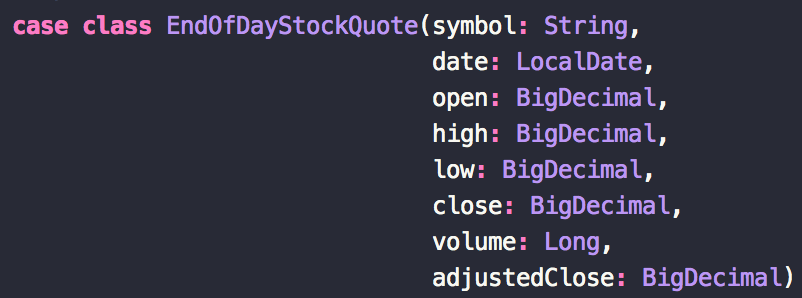
\includegraphics[max width=\textwidth]{endOfDayStockQuote}
  \end{center}
  \caption{The \texttt{EndOfDayStockQuote} data structure.}
\end{figure}

\subsection{Opinion Aggregation}

The opinion aggregation component contains sentiment analysis code, facilities to aggregate an accurate crowd-sourced sentiment towards a stock from microblog posts based on the \textit{CrowdIQ} model, and facilities to store and retrieve microblogs from our database.

\subsubsection{Setting Up Database Schema}

Similar to the pricing data component, we need to setup a table in HBase to store our microblog posts.
Recall from Figure~\ref{microblogPostSchema} that a microblog post table has the column families \texttt{base\_data} and \texttt{options}.
From the HBase shell, we execute the command ``\texttt{create 'stocktwits','base\_data','prices'}'' to create the table that will store all of our post data.

\subsubsection{Database Interactions}

In the same pattern as the pricing data component, we define a trait named \texttt{MicroblogDataSource} (see Figure~\ref{microblogDataSource}).
\texttt{MicroblogDataSource} contains a \texttt{query} method that allows you to perform a time range query on the set of posts.
The \texttt{HBaseMicroblogDataSource} class, which implements the contract laid out by \texttt{MicroblogDataSource}, implements the \texttt{query} method so that it retrieves the posts from a table (specified in the class' constructor) in our HBase database.
Additionally, the \texttt{HBaseMicroblogDataSource} contains a \texttt{write} function that will write a set of posts into the HBase table.

Our microblog post data from StockTwits that we received from our client is in the form of a CSV file.
We implemented a \texttt{CsvMicroblogDataSource} class that reads the posts from our CSV file, so that we can write them to our database with an instance of the \texttt{HBaseMicroblogDataSource}.

% Figure - microblogDataSource
\begin{figure}[h]
  \label{microblogDataSource}
  \begin{center}
    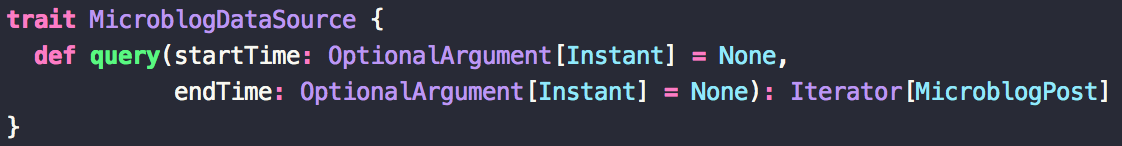
\includegraphics[max width=\textwidth]{microblogDataSource}
  \end{center}
  \caption{The \texttt{MicroblogDataSource} data structure.}
\end{figure}

\subsubsection{Sentiment Analysis}

The implementation of our sentiment analysis model is simply a slightly modified version of the code that was provided to us by our client Saurabh Chakravarty and his colleague Eric Williamson.
The provided sentiment analysis implementation used the Word2Vec feature extractor and the logistic regression classifier from Spark's MLlib \cite{sparkml}.
We trained and tested our sentiment analysis model using the posts from StockTwits that already had an author-specified bullish/bearish sentiment.
We sampled 50\% of the pre-classified posts to serve as the training data and the remaining pre-classified posts were used as testing data.

\subsubsection{Aggregation Model}

A class named \texttt{AggregatedOpinions} will be implemented to aggregate the sentiments towards each stock based on the method outlined in \textit{CrowdIQ} \cite{crowdiq}.
An instance of \texttt{AggregatedOpinions} is passed \texttt{MicroblogPost} objects (that include a sentiment that has been analyzed by our sentiment analysis model) one-by-one through a method named \texttt{on} (like an event listener).
The quantity of author individual weight times the degree of independence needs to be accumulated for each stock symbol and sentiment pair.
Therefore, with each post, \texttt{AggregatedOpinions} will accumulate these values in a map that is keyed by a tuple of the stock symbol and sentiment.
The degree of independence of a post is an exponential decay function that requires the order in which a post appears among others with the same sentiment and stock in a given time frame.
This requires an additional map (also keyed by a tuple of stock symbol and sentiment) to store the order in which the next post appears.
Individual weights for each author are also maintained in this object.
These weights are calculated by determining the post's score, which measures the accuracy of the prediction made by the post.
It does this by checking the price change of the stock in a time window after the post was made and checking if the trend is consistent with the prediction.
Therefore, to adjust the author weights, this object needs to store each post (using a queue) until after the time window when it can verify the price change.
The \texttt{AggregatedOpinions} class exposes a method named \texttt{sentimentForStock} which allows you to query for the aggregated sentiment of a stock in the current time window.
It also exposes a \texttt{reset} method which resets the time window (clears the current aggregated sentiments).

\subsection{Trading Simulation}

The implementation of the Trading Simulation component consists of the development of a virtual portfolio model, a trading context that collects events for a given time interval and passes them off to a trading strategy, and the trading strategies themselves.
This is quite an open-ended task.
Due to the complexity and importance of this component, which is required before we can implement and test any trading strategies that we encounter, all group members are responsible for contributing to this component.

\subsubsection{Virtual Portfolio}

The virtual portfolio stores a cash value as well as the number of each stock that you own.
It provides several functions that allow you to buy and sell shares of a stock.
Additionally, it performs error checking so that you cannot perform invalid trades.
Nick Anderson was responsible for implementing the first draft of the virtual portfolio.
After the first draft of the virtual portfolio was completed, our team convened to discuss the final form of this API.
This API consists of a class named \texttt{Portfolio} which stores the amount of cash available, and a map containing the stock symbols mapped to the amount of each stock that is currently held in the portfolio.
This class is modeled as an immutable object.
The \texttt{Portfolio} object requires a \texttt{StockPriceDataSource} instance to buy/sell stocks or calculate the total value of the portfolio.
A \texttt{TransactionError} object is defined to represent an error performing a transaction.
This error object contains the previous portfolio and an error message describing what went wrong.
The \texttt{Portfolio} object contains several methods to perform transactions, all of which return either a \texttt{TransactionError} or the resulting \texttt{Portfolio} object.
The methods that perform transactions include \texttt{with\-Shares\-At\-Target\-Amount}, \texttt{with\-Shares\-At\-Target\-Value}, \texttt{with\-Shares\-Purchased\-At\-Value}, \texttt{with\-Shares\-Purchased}, \texttt{with\-Shares\-Sold}, and \texttt{with\-All\-Shares\-Sold}.
The \texttt{with\-Shares\-At\-Target\-Amount} and \texttt{with\-Shares\-At\-Target\-Value} methods perform a transaction so that the number of shares or the total value of the shares for a particular stock is a particular value.
The \texttt{with\-Shares\-Purchased\-At\-Value} and \texttt{with\-Shares\-Purchased} methods will try to purchase more shares of a stock using the number of shares or the amount that you can buy with a dollar value, respectively.
The \texttt{with\-Shares\-Sold} method will try to sell a number of shares of a stock.
The \texttt{with\-All\-Shares\-Sold} will sell all shares in the portfolio.
 
\subsubsection{Trading Context}

We are required to be able to easily define different trading strategies and execute them by passing old trading events.
At the core of this functionality is a class named \texttt{TradingContext}, which contains a list of all the trading strategies to test and a list of the event emitters that will generate events to pass to the strategies.
The \texttt{TradingContext} is responsible for obtaining the trading events from the emitters and passing them to the strategies in order.
This class contains a \texttt{run} method that runs a simulation for a given time interval.
This calls on the event emitters to generate the events for the provided time interval and pass them off to all of the strategies.
Each trading strategy is implemented by extending a Scala trait named \texttt{TradingStrategy}.
This involves implementing an \texttt{on} method that responds to an instance of \texttt{TradingEvent}.
In this method, you can execute transactions on your portfolio or maintain information that influences the decision to perform a transaction (like analyzing the sentiment of a \texttt{MicroblogPost}).
The \texttt{TradingEvent} trait defines each event as containing a time (so that they can be sorted).
Extensions of \texttt{TradingEvent} can choose to provide more information.
For example, we define the \texttt{MicroblogPostEvent} as containing a \texttt{MicroblogPost} object.
The \texttt{TradingEventEmitter} trait allows you to define how events are generated by implementing an \texttt{eventsForInterval} method where you may return an interval of events for a given time interval.
In the \texttt{TradingStrategy}'s \texttt{on} method, we can use Scala's pattern matching feature as a convenient way to check the type of event and extract data from it.
Figures~\ref{tradingStrategy}, ~\ref{tradingEvent}, and ~\ref{microblogPostEvent} show our \texttt{TradingStrategy} trait, \texttt{TradingEvent} trait, and \texttt{MicroblogPostEvent} class, respectively.

% Figure - tradingStrategy
\begin{figure}[h]
  \label{tradingStrategy}
  \begin{center}
    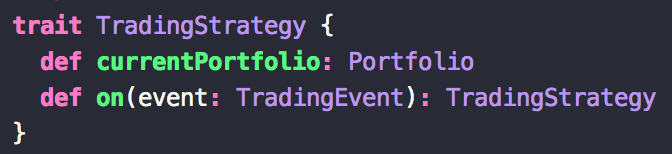
\includegraphics[max width=\textwidth]{tradingStrategy}
  \end{center}
  \caption{The \texttt{TradingStrategy} trait.}
\end{figure}

% Figure - tradingEvent
\begin{figure}[h]
  \label{tradingEvent}
  \begin{center}
    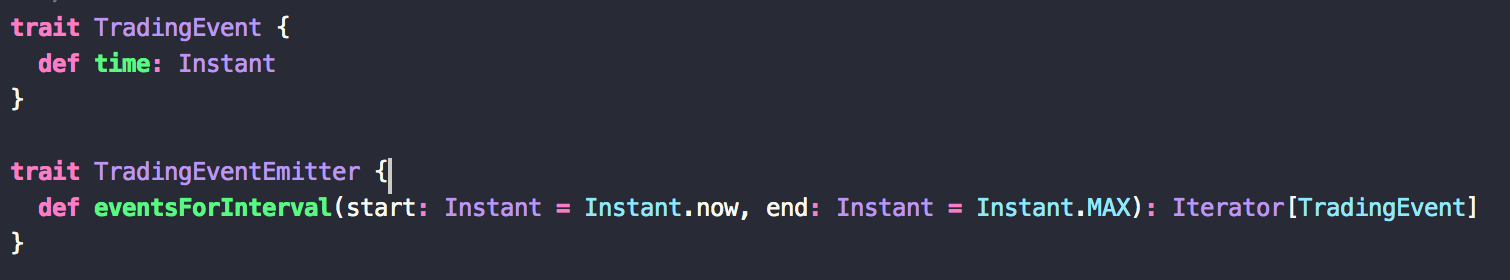
\includegraphics[max width=\textwidth]{tradingEvent}
  \end{center}
  \caption{The \texttt{TradingEvent} trait and the \texttt{TradingEventEmitter} trait.}
\end{figure}

% Figure - microblogPostEvent
\begin{figure}[h]
  \label{microblogPostEvent}
  \begin{center}
    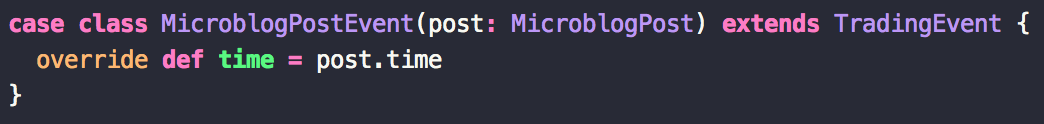
\includegraphics[max width=\textwidth]{microblogPostEvent}
  \end{center}
  \caption{A \texttt{TradingEvent} signifying a new microblog post was made.}
\end{figure}

\subsubsection{Trading Strategies}

Referring back to our timeline from the design report, we are planning to implement the trading strategy described by \textit{CrowdIQ} before March 15 \cite{crowdiq}.
We can run simulations with this strategy and compare the results achieved by our implementation to see our simulation software in action and to make sure that our implementation of \textit{CrowdIQ} is working properly.
More rigorous testing and analysis will be performed at later stages of the project.
Additionally, we will implement a simple strategy that invests in the S\&P 500 index fund to compare our results against the market performance.
The three trading strategies that we'd like to start implementing on April 1 will be implemented after we have ensured that we have a working system on which to test our strategies.
The intricate details of these strategies will be discussed in detail in the Refinement report.


%%% Local Variables:
%%% mode: latex
%%% TeX-master: "../report"
%%% End:
